\section{Design and Implementation}\label{sec:design_imple}
In this section, we present Linux-RTXG design and implementation.
Linux-RTXG is an abbreviation of Linux Real-Time eXtension including GPU resouce management,
which is Linux real-time GPU scheduling framework without kernel modification.

We describe the main contribution of the GPU scheduler and the integration to CPU scheduler in this paper.
CPU scheduling description is minimized because Linux-RTXG is based on RESCH.

%Linux-RTXGはLinux Real-Time eXtension included GPU resource managementの略称であり、Linuxのリアルタイム拡張に加えてGPUのResourceマネージメントを行うためのフレームワークである。
%Linux-RTXGはベースとしてRESCHを用いているため、CPUスケジューラに関する記述は最小限に抑え、
%本論文の大筋である、GPUスケジューラをメインに、CPUスケジューラとの統合といった部分を記載していく。

\subsection{Linux-RTXG}
\begin{figure}[t]
\begin{center}
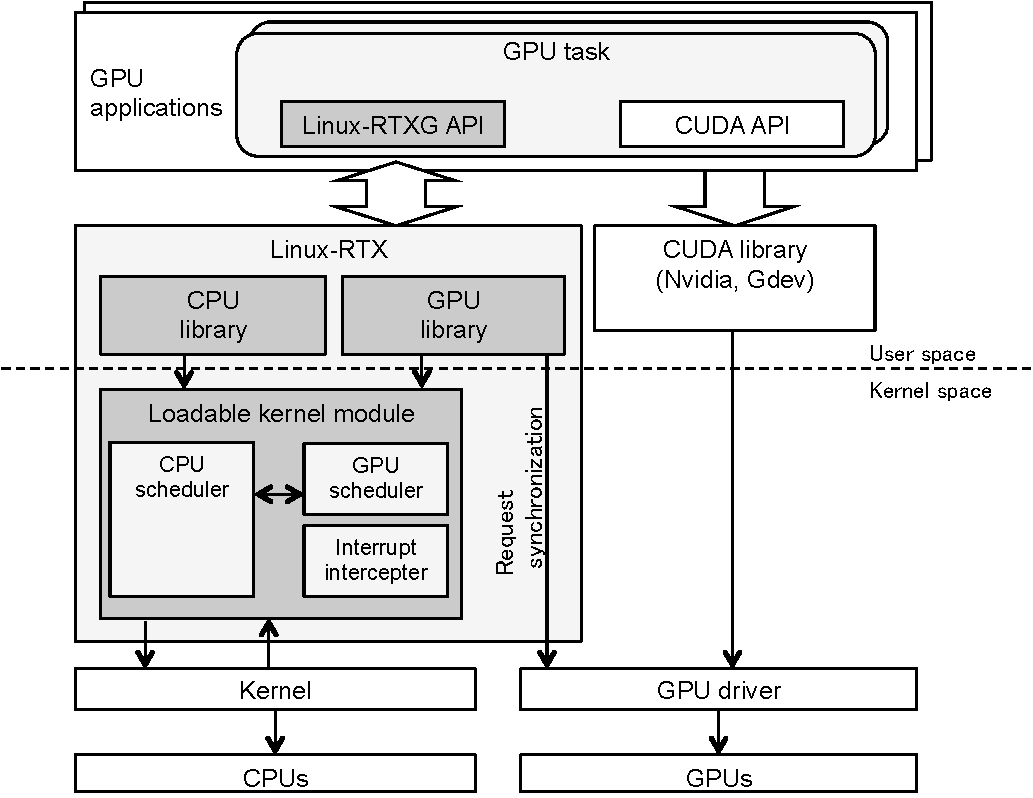
\includegraphics[width=0.35\textwidth]{img/overview.pdf}
\caption{Overview of the Linux-RTXG}
\label{fig:overview}
\end{center}
\end{figure}

Figure~\ref{fig:overview} shows an overview of Linux-RTXG.
Linux-RTXG is divided into two parts: a Linux-RTXG core and a Linux-RTXG library.
The Linux-RTXG core has a CPU task scheduler, a GPU task scheduler, and a GPU resource reservation mechanism.
Because the Linux-RTXG core is loaded into the kernel-space, it can use the kernel exported functions such as $schedule()$, $mod\_timer()$, $wake\_up\_process()$ and $set\_cpus\_allowed\_ptr()$.

The Linux-RTXG library is interface to communicate between application and Linux-RTXG core.
These interface are implemented using an ioctl system call, which is a standard way of communicating to a driver.

The part of the library included a method that is an independent synchronization method.
The independent synchronization method is used only on the Nvidia driver.
In case of using an open-source GPU driver such as Nouveau~\cite{nouveau}, GPU runtime must use part of Gdev.
Because Gdev can manage arbitrary interrupt of the GPU kernel in the user-space mode, the GPU scheduler have not need the independent synchronization method because 

\subsection{GPU Scheduling}
\begin{table*}[t]
\begin{center}
\caption{Basic Linux-RTXG APIs}
\label{tab:rtx-api}
\begin{tabular}{|l|p{50em}|} \hline
rtx\_gpu\_open() & To register itself to Linux-RTXG, and create scheduling entity. It will must call first. \\ \hline
rtx\_gpu\_device\_advice() & To get the recommendation of GPU devices to be used \\ \hline
rtx\_gpu\_launch() & To control the GPU kernel launch timing, in other words it is scheduling entry point. It will must call before the CUDA launch API. \\ \hline
rtx\_gpu\_sync() & To wait for finishing GPU kernel execution by sleeping with TASK UNINTERRUPTIBLE status.\\ \hline
rtx\_gpu\_notify() & To send the notify/fence command to GPU microcontroller. The fence or the notify is selected flag is set by argument.\\ \hline
rtx\_gpu\_close() & To release scheduling entity.\\ \hline
\end{tabular}
\end{center}
\end{table*}

Linux-RTXG is API-driven scheduler where the scheduler invoked only when computation requests are submitted.
The basic APIs supported by Linux-RTXG are listed in Table~\ref{tab:rtx-api}.
Some APIs have arguments and the others do not.
Linux-RTXG does not modify the existing CUDA API to cope with proprietary software to be independent from the runtime.
However, user has to add Linux-RTXG API to existing CUDA application for using the Linux-RTXG scheduler.

The sample code of using the Linux-RTXG scheduler is shown in Figure~\ref{fig:sample},
and its code except GPU scheduling is omitted.
GPU tasks may be provided with a function by calling Linux-RTXG's API at strategic points.

\begin{figure}[t]
\begin{center}
\begin{tabular}{l}
\hline\hline
{\scriptsize \verb|void gpu_task(){        |}\\
{\scriptsize \verb| /* variable initialization  */        |}\\
{\scriptsize \verb| /* calling RESCH API */        |}\\
{\scriptsize \verb|  dev_id = rtx_gpu_device_advice(dev_id); |}\\
{\scriptsize \verb|  cuDeviceGet(&dev, dev\_id);           |}\\
{\scriptsize \verb|  cuCtxCreate(&ctx, SYNC_FLAG, dev);    |}\\
{\scriptsize \verb|  rtx_gpu_open(&handle, vdev_id);     |}\\
{\scriptsize \verb| /* Module load and set kernel function */ |}\\
{\scriptsize \verb| /* Device memory allocation        */ |}\\
{\scriptsize \verb| /* Memory copy to device from host */ |}\\
{\scriptsize \verb|  rtx_gpu_launch(&handle); |}\\
{\scriptsize \verb|  cuLaunchGrid(function, grid_x, grid_y); |}\\
{\scriptsize \verb|  rtx_gpu_notify(&handle); |}\\
{\scriptsize \verb|  rtx_gpu_sync(&handle);   |}\\
{\scriptsize \verb|  /* Memory copy to host from device */  |}\\
{\scriptsize \verb|  /* Release allicated memory */  |}\\
{\scriptsize \verb|}|}\\
\hline\hline
\end{tabular}
\caption{sample code of using Linux-RTXG scheduler}
\label{fig:sample}
\end{center}
\end{figure}

\begin{figure}[t]
\begin{center}
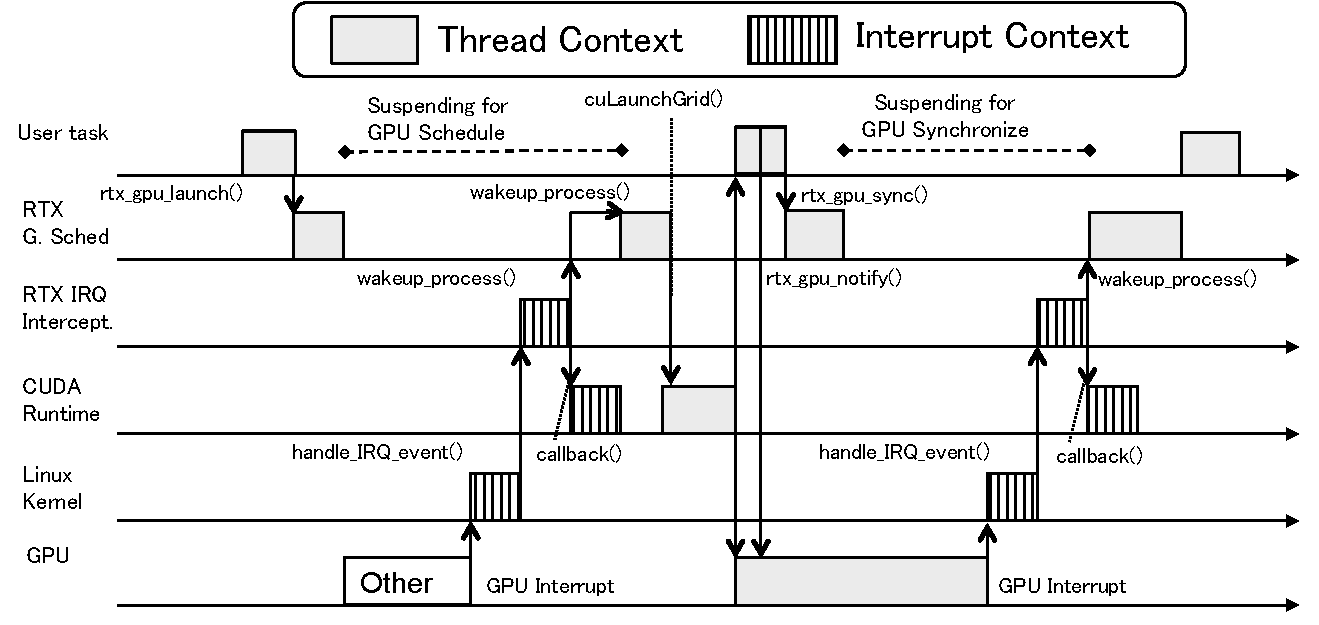
\includegraphics[width=0.5\textwidth]{img/gsched_controlflow.pdf}
\caption{GPU Scheduling control flow}
\label{fig:controlflow}
\end{center}
\end{figure}


Figure~\ref{fig:controlflow} shows the control flow of the sample code.
The configuration is the Kernel issue that is restricted to single kernel.
A GPU Task can control the timing of GPU kernel execution by calling $rtx\_gpu\_launch()$.
The task goes to sleep until the wakeup by interrupt why the task is not permitted issuance of GPU kernel due to already execute other task in the GPU.
%The configure is limited to one of  issuance of GPU kerlenel GPUカーネルの発行はひとつに制限されており、すでにGPUでタスクがうごいている状態とし、同期は割込みを用いたNOTIFYによって行うものとする。
%ユーザタスクは$rtx_gpu_launch()$を呼び出すことで、GPUカーネル実行のタイミングをコントロールすることができる。
%既にGPUでタスクが動いており、現在カーネル発行を許可されているタスクが自身でないため、割込みによって起床されるまでtask uninterruptible状態で自らスリープに入る。

%立ち上がって眠るところまでの説明
Other task's GPU kernel is finishied, 
then, linux kernel handle the interrupt.
The interrupt intercepter wakeup the GPU scheduler (RTX G. Sched. in Figure~\ref{fig:controlflow}) by intercept interrupt.
The GPU scheduler wakeup the sleeping task.
The waken up the task issue the GPU kernel via CUDA API such as $cuLaunchGrid()$.
%e the interrupt interceptor wakeup the GPU scheduler, GPU scheduler wakeup the sleeping task. 
After the GPU kernel issued, task register the NOTIFY for occurring the interrupt,
and task to sleep until it occurs interrupt.
To pick up the next task is performed by the GPU scheduler caused by interruption of GPU kernel finish.
Linux-RTXG is doing the execution order control tasks in the above flow.
%動いていたタスクが終了した時点で割込みが発行され、そのコンテキストのInterrupt intercepterによってスリープしていた次のタスクが起床される。
%起床したタスクは$cuLaunchGrid()$などのCUDA APIを通じてGPUカーネルの発行を行う。
%カーネル発行後、割込みを発生させるためのNotifyの登録を行い、その割込みが発生するまでスリープに入る。
%割込みが発生すると次のタスクが動作するといったフローを持ってスケジューリングが行われる。
%次のタスクの選択は、割込みによって起こされるGPU schedulerによって行われる。

We present hierarchal scheduling included group (virtual GPU) scheduling and GPU kernel scheduling.
The virtual GPU scheduling uses a resource reservation mechanism.
The GPU kernel scheduling uses  a priority scheduling.
Specifically, GPU kernel execution is associated to each scheduling entity while Linux-RTXG grouped the scheduling entity to virtual GPUs.
The virtual GPUs belong to any of physical GPUs.
In Linux-RTXG, resources are distributed in its virtual GPUs.

Figure~\ref{fig:scheduling} shows pseudo-code of scheduling mechanism.
$on\_arrival$ is called when a GPU task is requested GPU kernel launch issue.
In $on\_arrival$, a GPU task to check whether the given execute permission to virtual GPU of task itself, and then, check the se permit.
If a virtual GPU to which the GPU task belongs has not executing permission, the GPU task is enqueued to wait\_queue and goes to sleep.
On the other hand, if the virtual GPU has executing permission, the GPU task goes to launch issue.

$on\_completion$ is called by a scheduler thread, when the GPU kernel is completion.
$on\_completion$ picks up the next virtual GPU and the next a GPU task.
Next then, $on\_completion$ wakes up the pick uped the GPU task.

%このグループに対して資源の配布 (スケジューリングスレッドによって一定周期で補充)を行い,
%グループ毎に実行許可をスケジューリングポリシー (e.g. BAND, Credit)に従い与えていく.
%GPUタスクは自身のコンテキストが所属するグループに実行許可が与えられているかを確認し実行を行う.
%次タスクの選択はグループ,グループ内のコンテキストと階層的に選択することで,リザベーションに加え優先度スケジューリングとより自由度の高いスケジューリングメカニズムを提供する.
\begin{figure}[t]
\begin{center}
\begin{tabular}{l}
\hline
{\scriptsize \verb| se: The scheduling entity |}\\
{\scriptsize \verb| se->vgpu: The group that is belonged se|}\\
{\scriptsize \verb| se->task: The task that is associated with se |}\\
{\scriptsize \verb| vgpu->parent: The physical GPU identification|}\\
\hline
{\scriptsize \verb|void on_arrival(se) {|}\\
{\scriptsize \verb| check_permit_vgpu(se->vgpu)    |}\\
{\scriptsize \verb| while(!check_permit_se(se)){|}\\
{\scriptsize \verb|   enqueue(se->vgpu,se); |}\\
{\scriptsize \verb|   sleep_task(se->task); |}\\
{\scriptsize \verb| }|}\\
{\scriptsize \verb|}|}\\
{\scriptsize \verb|void on_completion(se) {|}\\
{\scriptsize \verb| reset_the_permit(se->vgpu, se)|}\\
{\scriptsize \verb| n_vgpu = pick_up_the_next_vgpu(se->vgpu->parent) |}\\
{\scriptsize \verb| se = pick_up_the_next_se(n_vgpu)|}\\
{\scriptsize \verb| if(se) {|}\\
{\scriptsize \verb|   dequeue(se->vgpu,se);|}\\
{\scriptsize \verb|   wakeup_task(se->task);|}\\
{\scriptsize \verb| }|}\\
{\scriptsize \verb| set_the_permit(se->vgpu, se)|}\\
{\scriptsize \verb|}|}\\
\hline
\end{tabular}
\caption{High Level Pseudo-code of scheduling mechanisms}
\label{fig:scheduling}
\end{center}
\end{figure}

\subsection{GPU synchronization}
We describe the independent synchronization mechanism and the interrupt intercept.
The independent synchronization mechanism is occuring NOTIFY and FENCE without using GPU runtime's API.
The interrupt intercept is to realize interrupt-driven wakeup the scheduler without kernel modification.
%で説明したruntime environmentに依存しない同期の実現と
%interrupt-drivenなスケジューラ起床を実現するために,kernel freeなまま同期に用いるinterruptを取得するinterrupt interceptを実装する.
Linux-RTXG uses the independent synchronization mechanisms as much as possible,
because we do not want using black-box resource management to realize truly real-time resource environments.

%ラウンチされたカーネルが終了したタイミングをスケジューラはNOTIFYかFENCEによって取得する。
%本ワーカースレッドは実行中のカーネルが終了した時点で次のタスクの選択を行う。
%ワーカースレッドはタスクの選択後にCPU資源を他のタスクに明け渡すためにサスペンドに入る。

\textbf{Independent synchronization mechanism from runtime}
We present an independent synchronization mechanism of the NOTIFY and the FENCE.
The mechanism is to occur interrupt for NOTIFY, and to write the fence value by microcontrollers for FENCE.
NVIDIA's proprietary software uses ioctl interface to communicate between kernel-space and user-space.
These ioctl interfaces are provided drivers function such as device memory allocation, get the GPU information and memory mapping.
Gdev build infrastructure that is able to execute on the NVIDIA's driver using these ioctl interfaces.

We also use this ioctl interface similar to Gdev's command sending method for our method.
Specifically, our method is divided into two parts: Initialize and Notify.
%我々はGdevと同様のアプローチでコマンドをSendingする.
%ここでは、ランタイムから独立した割込み機構として、独自にNOTIFY、FENCEに用いるsignを発生させる仕組みを提供する。
%ここでのsignは、NOTIFYは割込み、FENCEはmappedメモリへの値の書き込みである。
%NVIDIAのクローズドソースドライバはNouveauプロジェクトのリバースエンジニアリングによる解析によって、ioctlを使ったインタフェースになっていることがわかっている。
%Gdevではこの解析された情報を用いて、NVIDIAのクローズドソースドライバとオープンソースライブラリという掛け合わせでCUDAを実行できる基盤が構築されている。
%This method 
%本メソッドは大きく2つに分かれ、それぞれInitializeとNotifyと呼ぶ。
Initialize processes for generating a GPU context dedicated this method.
These processes are included a creating virtual address space, a allocating indirect buffer object for command sending, and a creating context object.
The virtual address space is used for managing the GPU device memory space and kernel memory space (Host-side) such as indirect buffer.
The indirect buffer is an area of storing GPU commands for sending GPU commands.
The creating context object is preparation for using the FIFO engine,
such as allocating kernel memory object and mapping FIFO engine register to host memory space by memory-mapped I/O.
The FIFO engine is GPU microcontroller for receiving commands.
The Notify processes send commands to the compute engine or the copy engine by iowrite commands to mapped FIFO engine's register.
%Initializeは、いわゆるコンテキストの生成に値する。Virtual Address Spaceやコマンド送信に用いるIndirect Bufferの確保、コンテキストオブジェクトの生成などを行う。
%NotifyはComputeエンジンやCopyエンジンに向けて割込み発生、もしくはFENCE用に値の書き込みを行うコマンドを送信する。
This independent generating synchronization sign for synchronization mechanisms is using reverse engineering.
However, the method has limitation because the method depends on the proprietary runtime environment.

%本アプローチに用いるインタフェースは公式にサポートされていないために、ベンダーによる急な仕様変更には対応できない。
%しかしながら、これ以外に割込みを発生させるアプローチがなく、クローズドソースを用いた場合の限界であるといえる。

\textbf{Interrupt interception:}
Interrupts are handled by the ISR (Interrupt Service Routine) that is registered kernel by the device driver.
In addition, scheduler require to identify the interrupt by using readling GPU status register.
It must be done before original ISR is reset the GPU status register.

%割込みはデバイスドライバ(カーネルと共にパッケージされている)によって登録されたISRがハンドルする。
%加えて、割込みの識別はGPUのステータス・レジスタを読み込んで行う必要があり、
%GPUドライバが割込みレジスタをリセットする前に、実行される必要がある。
The Linux kernel has structures that holds the interrupt parameters called irq\_desc for each interrupt number.
These structures have structures called irq\_action including the ISR callback pointer.
irq\_desc is allocated to global memory space of the kernel, anyone is accessible from kernel space.
Linux loadable kernel modules can get an irq\_desc for running in kernel, while also can get a callback pointer of ISR.
We retain getting the callback pointer of a GPU device driver's ISR, and then we register a interrupt interception ISR to kernel.
So, we get the interrupt interception by the interrupt interception ISR and calling retaining callback pointer.
%Linuxでは、割込み番号ごとにirq\_descという割込みのパラメータを保持する構造体を持っている。
%この構造体にはISRの関数ポインタを含むirq\_actionという構造体がリストで接続されている。
%irq\_descはグローバルな領域に確保されており、カーネル空間からであれば誰でも参照可能である。
%Linuxのローダブルカーネルモジュールはカーネル空間で動作しているため、このirq\_descを取得でき、
%Interrupt handlerの関数ポインタも取得可能である。
%我々はこの取得した関数ポインタを保持し、我々の傍受用ISRをカーネルに登録する。
%そして傍受用ISRで、事前に保持しておいたGPUドライバの割込みハンドラの関数コールバック関数として呼び出すことで、通常の割込みハンドリングを実行する。
In addition, I/O registers are mapped to kernel memory space by device driver from the PCIe base address registers (BARs)~\cite{fujii:icpads2013,kato2013zero}.
Therefore, Linux-RTXG remaps the BAR0 to our allocated space by using $ioremap()$ when the ISR is initializes.
The interrupt interception identifies interrupt by reading the mapped-space.

%加えて我々のこれまでの研究\cite{fujii:icpads2013,kato2013zero}で、GPUのio registerはPCIeのBAR0によって指定されたアドレスから存在しておりカーネル空間にデバイスドライバによってマッピングされていることがわかっている。
%そのためLinux-RTXGが傍受用ISRの初期化の際に$ioremap()$によってBAR0空間をマッピングしておき、傍受用ISRが呼び出された際にマッピングされたレジスタを読み込むことで、
%割込みの識別を行う。
\subsection{Scheduler Integration}
Linux scheduler has various real-time scheduling policies that were $SCHED\_DEADLINE$, $SCHED\_FIFO$ and $SCHED\_RR$.
$SCHED\_DEADLINE$ is implementation of Constant Bandwidth Server and Global Earliest Deadline First,
while $SCHED\_DEADLINE$ is included in mainline of Linux 3.14.0 kernel.
%特にSCHED\_DEADLINEはLinux 3.14よりメインラインに含まれたConstant Bandwidth ServerとGlobal-EDFの実装であり、
%Linuxをリアルタイム拡張するにおいて有効に利用できるクラスである。
However, synchronization does not work well in a SCHED\_DEADLINE scheduling policy when using GPU tasks.

This problems are twofold.
The first is implementation of sched\_yield---in kernel space used yield()---.
The second is implementation of return from sleeping state.

%本問題は2種類存在しており、
%sched\_yield()によるCPU放棄の実装によるものと、%suspendingした後の復帰の実装によるものである。

The first problem occurs by releasing the CPU using $sched\_yield()$ when waiting for I/O in polling.
Polling (Spin) is the exclusive CPU, therefore a task may once better to release the CPU can obtain good results.
However, sched\_yield will set 0 to polling task's runtime of remaining execution time treated as a parameter of $SCHED\_DEADLINE$.
%一つ目のsched\_yield(カーネル内ではyield関数)は、FENCEのようにPollingされる場合に生じる。
%pollingはCPUを専有してしまう方式であり、他のタスクへの影響を考えた場合、一度CPUを放棄したほうが良い結果が得られる場合がある。
%しかしながらsched\_yieldでは、SCHED\_DEADLINEの内部パラメータとして扱う、runtime(残りの実行しても良い時間)を0にしてしまう。
Thereby, the task can not execute until runtime is replenished in the next period.
Therefore, the task is unable to call $sched\_yield()$ between polling.
%これによって、次の周期が訪れるまではruntimeが補充されることがなく、そのタスクは実行権限を失う。
The $sched\_yield()$ is used much by device drivers and library as well as GPU runtime.
These software is affected by this problems.
Even NVIDIA CUDA is affected depending on the setting.
We support this problem by limit the GPU synchronization method to NOTIFY  in the $SCHED\_DEADLINE$ policies.
%Linux-RTXGではSCHED\_DEADLINE時はNOTIFYを使うことを推奨し、sched\_yieldの利用を制限することで対応した。
%sched\_yieldはGPUランタイムに限らず、デバイスドライバやライブラリなどで多く利用されており、
%それら全てで、SCHED\_DEADLINEポリシー上では正常に動作しない結果が生じる可能性が高い。
%NVIDIAのCUDAにおいても同期フラグの設定次第で本問題に影響を受ける。

The second problem is subjected to a check equation (1) when restore task from sleeping state.
If equation (1) is true, runtime is replenished and absolute deadline is setted next cycle deadline.
%2つ目の問題はタスクが一度sleeping状態に入り、復帰時に式(1)を用いて実行可能性についてチェックを行う。
%式(1)が真の時、runtimeが補充され、absolute deadlineが次の周期に設定される。

{\scriptsize
\begin{equation}
\frac{Absolute\_Deadline - Current\_Time}{Remaining\_Runtime} > \frac{Relative\_Deadline}{Period}
\end{equation}
}

We support this check by
subtracting the GPU execution time from $Remaining\_Runtime$
when task is restored by GPU kernel execution with the exception of the task is restored by period.
%Linux-RTXGでは本チェックについて、sleeping状態から起床するという状態を、
%GPUカーネル実行による復帰と、周期による復帰とで種類分けし、
%GPUカーネル実行による復帰時にのみ、$Remaining\_Runtime$からGPU execution timeを引くことで対応した。

